\begin{frame}
	\frametitle{Execution time of code generator (sampling rate 1000)}

	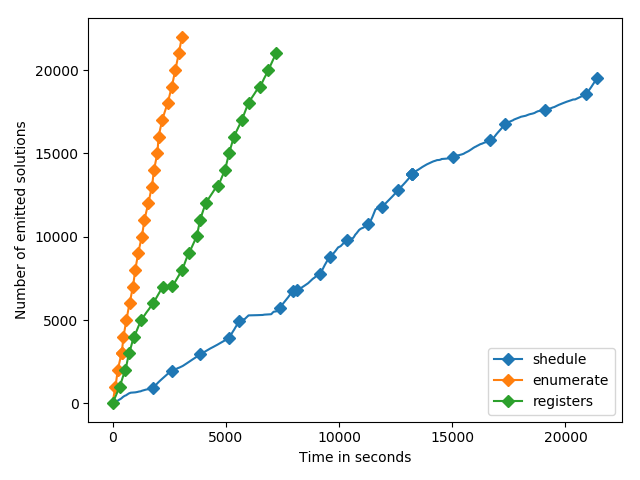
\includegraphics[width=\textwidth]{../results/figures/generator_time}

\end{frame}

\begin{frame}
	\frametitle{Estimated execution time}

	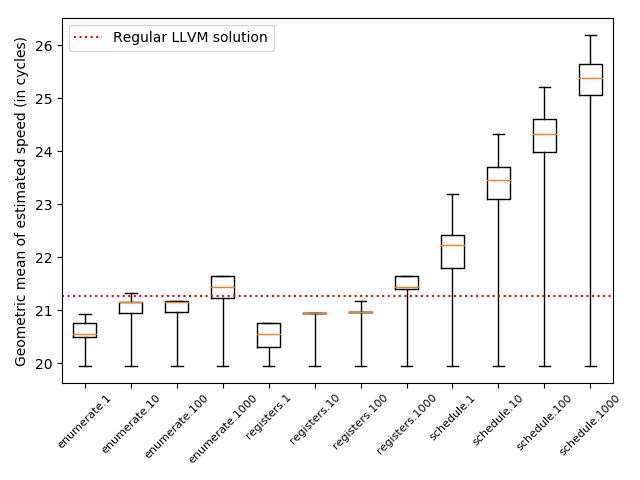
\includegraphics[width=\textwidth]{../results/figures/cost_speed}

\end{frame}

\begin{frame}
	\frametitle{Surviving gadgets}

	\adjincludegraphics[width=\textwidth,trim={0 {0.5\height} 0 0},clip]{../results/figures/gadgets}

\end{frame}

\begin{frame}
	\frametitle{Surviving gadgets cont.}

	\adjincludegraphics[width=\textwidth,trim={0 0 0 {0.5\height}},clip]{../results/figures/gadgets}

\end{frame}

\begin{frame}
	\frametitle{Shortcomings}

	Data set. \textcite{large-scale-automated} found 433.milc from SPEC2006 to be representative
	in terms of gadgets

	\vspace{0.5cm}

	Not on x86

\end{frame}
